
        \documentclass[addpoints,spanish, 12pt,a4paper]{exam}
        %\documentclass[answers, spanish, 12pt,a4paper]{exam}
        
        \pointpoints{punto}{puntos}
        \hpword{Puntos:}
        \vpword{Puntos:}
        \htword{Total}
        \vtword{Total}
        \hsword{Resultado:}
        \hqword{Ejercicio:}
        \vqword{Ejercicio:}

        \usepackage[utf8]{inputenc}
        \usepackage[spanish]{babel}
        \usepackage{eurosym}
        %\usepackage[spanish,es-lcroman, es-tabla, es-noshorthands]{babel}


        \usepackage[margin=1in]{geometry}
        \usepackage{amsmath,amssymb}
        \usepackage{multicol, xparse}

        \usepackage{yhmath}

        \usepackage{verbatim}
        %\usepackage{pstricks}


        \usepackage{graphicx}
        \graphicspath{{../img/}}




        \let\multicolmulticols\multicols
        \let\endmulticolmulticols\endmulticols
        \RenewDocumentEnvironment{multicols}{mO{}}
         {%
          \ifnum#1=1
            #2%
          \else % More than 1 column
            \multicolmulticols{#1}[#2]
          \fi
         }
         {%
          \ifnum#1=1
          \else % More than 1 column
            \endmulticolmulticols
          \fi
         }
        \renewcommand{\solutiontitle}{\noindent\textbf{Sol:}\enspace}

        \newcommand{\samedir}{\mathbin{\!/\mkern-5mu/\!}}

        \newcommand{\class}{1º Bachillerato}
        \newcommand{\examdate}{\today}

        %\newcommand{\tipo}{A}


        \newcommand{\timelimit}{80 minutos}

        \renewcommand{\solutiontitle}{\noindent\textbf{Solución:}\enspace}


        \pagestyle{head}
        \firstpageheader{
\includegraphics[width=0.2\columnwidth]{header_left}}{\textbf{Departamento de Matemáticas\linebreak \class}\linebreak \examnum}{
\includegraphics[width=0.1\columnwidth]{header_right}}
        \runningheader{\class}{\examnum}{Página \thepage\ of \numpages}
        \runningheadrule
        
        \pointsinrightmargin % Para poner las puntuaciones a la derecha. Se puede cambiar. Si se comenta, sale a la izquierda.
        \extrawidth{-2.4cm} %Un poquito más de margen por si ponemos textos largos.
        \marginpointname{ \emph{\points}}

        \printanswers
            \newcommand{\tipo}{A}\newcommand{\examnum}{Final 3ª evaluación}
        \begin{document}
        \noindent
        \begin{tabular*}{\textwidth}{l @{\extracolsep{\fill}} r @{\extracolsep{6pt}} }
        \textbf{Nombre:} \makebox[3.5in]{\hrulefill} & \textbf{Fecha:}\makebox[1in]{\hrulefill} \\
         & \\
        \textbf{Tiempo: \timelimit} & Tipo: \tipo 
        \end{tabular*}
        \rule[2ex]{\textwidth}{2pt}
        Esta prueba tiene \numquestions\ ejercicios. La puntuación máxima es de \numpoints. 
        La nota final de la prueba será la parte proporcional de la puntuación obtenida sobre la puntuación máxima. 

        \begin{center}


        \addpoints
             %\gradetable[h][questions]
            \pointtable[h][questions]
        \end{center}

        \noindent
        \rule[2ex]{\textwidth}{2pt}

        \begin{questions}

%        \question Calcula los siguientes límites:
%        \begin{multicols}{1}
%        \begin{parts} \part[1] $$\lim_{x \to 3}\left(\frac{3 x^{2} - 11 x + 6}{x^{3} - 3 x^{2} + x - 3}\right)$$  \begin{solution}   $\frac{7}{10}$   \end{solution} \part[1] $$\lim_{x \to \infty} e^{1 - x}$$  \begin{solution}   $0$   \end{solution} \part[1] $$\lim_{x \to -2}\left(\frac{x^{3} + x^{2} - x + 2}{x^{2} + 4 x + 4}\right)$$  \begin{solution}   No existe el límite   \end{solution} \part[2] $$\lim_{x \to 2} \left(\frac{x^{3} - 4}{x^{2}}\right)^{\frac{1}{x - 2}}$$  \begin{solution}   $e^{2}$   \end{solution}
%        \end{parts}
%        \end{multicols}
        
        \question Calcula los siguientes límites:
        \begin{multicols}{1}
        \begin{parts} \part[1] $$\lim_{x \to 2}\left(\frac{x^{3} - 2 x^{2} + 2 x - 4}{3 x^{2} - 8 x + 4}\right)$$  \begin{solution}   $\frac{3}{2}$   \end{solution} \part[1] $$\lim_{x \to -\infty} e^{x - 1}$$  \begin{solution}   $0$   \end{solution} \part[1] $$\lim_{x \to -1}\left(\frac{x^{3} + 1}{x^{2} + 2 x + 1}\right)$$  \begin{solution}   No existe el límite   \end{solution} \part[2] $$\lim_{x \to 3} \left(\frac{x^{2} - x}{x + 3}\right)^{\frac{1}{x - 3}}$$  \begin{solution}   $e^{\frac{2}{3}}$   \end{solution}
        \end{parts}
        \end{multicols}
        
        
        
%        \question Dada la función:$f(x)=\frac{x^{2} - 2 x + 1}{2 x + 3}$, calcular:
%        \begin{multicols}{1}
%        \begin{parts} \part[1] Dominio de $f(x)$  \begin{solution}   $Dom(f)=\left(-\infty, - \frac{3}{2}\right) \cup \left(- \frac{3}{2}, \infty\right)$\\ \resizebox{0.4\textwidth}{!}{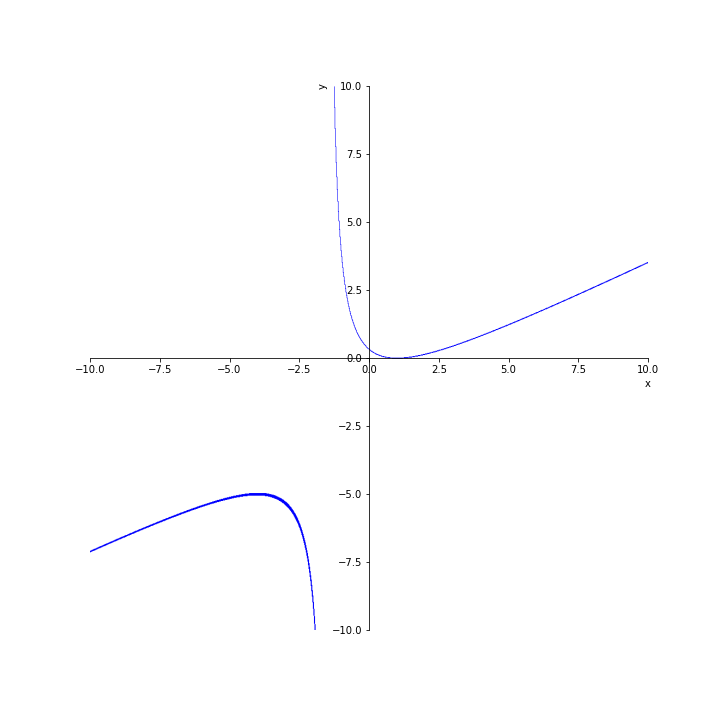
\includegraphics[width=1\columnwidth]{fin301-0}}   \end{solution} \part[2] Asíntotas verticales, horizontales y oblicuas, en caso que existan  \begin{solution}   Asíntotas:\\A.V. $x=-3/2$\\A.O. $y=\frac{x}{2} - \frac{7}{4}$ \\A.O. $y=\frac{x}{2} - \frac{7}{4}$ \\   \end{solution}
%        \end{parts}
%        \end{multicols}
%        \question Dada la función:$f(x)=\frac{- x^{2} - x + 3}{x^{2} + x - 2}$, calcular:
%        \begin{multicols}{1}
%        \begin{parts} \part[1] Dominio de $f(x)$  \begin{solution}   $Dom(f)=\left(-\infty, -2\right) \cup \left(-2, 1\right) \cup \left(1, \infty\right)$\\ \resizebox{0.4\textwidth}{!}{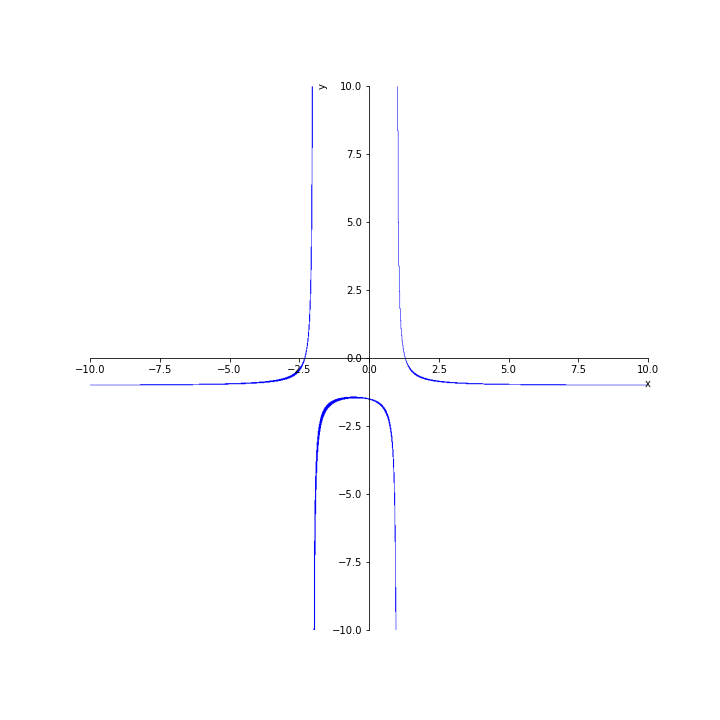
\includegraphics[width=1\columnwidth]{fin301-1}}   \end{solution} \part[2] Asíntotas verticales, horizontales y oblicuas, en caso que existan  \begin{solution}   Asíntotas:\\A.V. $x=-2$\\, A.V. $x=1$\\A.H. $y=-1$\\A.H. $y=-1$\\A.O. $y=-1$ \\A.O. $y=-1$ \\   \end{solution}
%        \end{parts}
%        \end{multicols}


        \question Dada la función:$f(x)=\sqrt{\frac{x}{x - 1}}$, calcular:
        \begin{multicols}{1}
        \begin{parts} \part[1] Dominio de $f(x)$  \begin{solution}   $Dom(f)=\left(-\infty, 0\right] \cup \left(1, \infty\right)$\\ \resizebox{0.4\textwidth}{!}{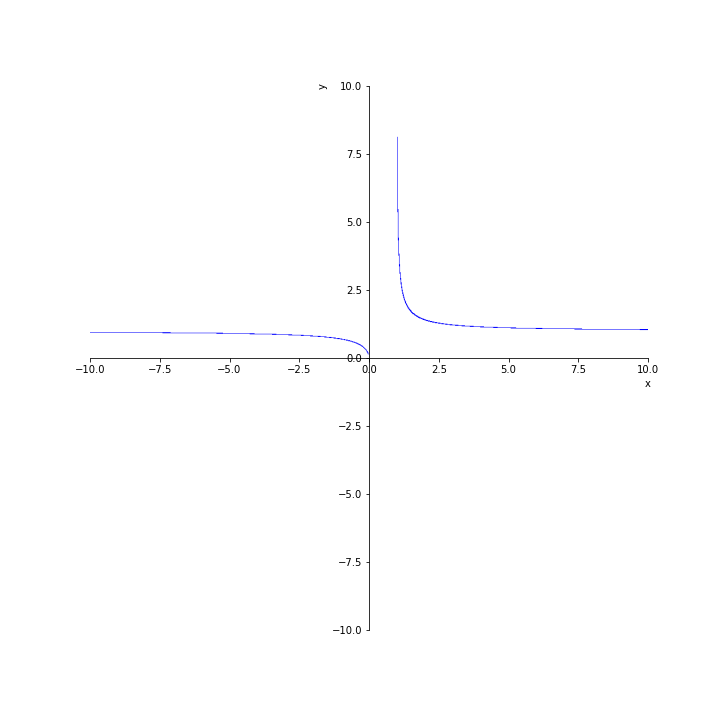
\includegraphics[width=1\columnwidth]{fin301-2}}   \end{solution} \part[2] Asíntotas verticales, horizontales y oblicuas, en caso que existan  \begin{solution}   Asíntotas:\\A.V. $x=1$\\A.H. $y=1$\\A.H. $y=1$\\A.O. $y=1$ \\A.O. $y=1$ \\   \end{solution}
        \end{parts}
        \end{multicols}


%        \question Estudia en qué puntos de $\mathbb{R}$ la función no es continua: 
%        \begin{multicols}{1}
%        \begin{parts} \part[2] $f(x)=\begin{cases} \frac{2 x^{2} + 7 x + 3}{x^{2} - 9} & \text{si}\: x \leq -2 \\\frac{\sqrt{x + 3} - 1}{x^{2} + 2 x} & \text{si} \: x > -2\end{cases}$  \begin{solution}   Singularidades de las expresiones analíticas: $\left\{-3, 0\right\}$.\\ Posibles discontinuidades en los extremos de los trozos:-2.\\En -2 no es continua porque no existe límite. Límites laterales: $\frac{3}{5}$ y $- \frac{1}{4}$   \end{solution}
%        \end{parts}
%        \end{multicols}
        
        
        \question Estudia en qué puntos de $\mathbb{R}$ la función no es continua: 
        \begin{multicols}{1}
        \begin{parts} \part[2] $f(x)=\begin{cases} \frac{x^{2} - 4}{x^{2} - 3 x + 2} & \text{si}\: x < 2 \\4 & \text{si}\: 2\leq x < 5 \\e^{x - 5} + 3 & \text{si}\: x > 5 \end{cases}$  \begin{solution}   Singularidades de las expresiones analíticas: $\left\{1\right\}$.\\ Posibles discontinuidades en los extremos de los trozos:2, 5.\\En 2 es continua ya que hay límite y $\lim = f(2)=4$. \\En 5 es continua ya que hay límite y $\lim = f(5)=4$   \end{solution}
        \end{parts}
        \end{multicols}
        
%        \question Halla a y b de modo que las siguientes funciones sean continuas:
%        \begin{multicols}{1}
%        \begin{parts} \part[2] $$f(x)=\begin{cases} a + e^{x + 2} & \text{si}\: x \leq -2 \\\frac{x + 1}{3 - x} & \text{si}\: -2 < x < 1 \\b x + 3 & \text{si}\: x \geq 1 \end{cases}$$  \begin{solution}   $\left\{ a : - \frac{6}{5}, \  b : -2\right\}$   \end{solution}
%        \end{parts}
%        \end{multicols}
        
        \question Halla a y b de modo que las siguientes funciones sean continuas:
        \begin{multicols}{1}
        \begin{parts} \part[2] $$f(x)=\begin{cases} a + e^{x + 3} & \text{si}\: x \leq -3 \\\frac{x + 2}{4 - x} & \text{si}\: -3 < x < 1 \\b x + 6 & \text{si}\: x \geq 1 \end{cases}$$  \begin{solution}   $\left\{ a : - \frac{8}{7}, \  b : -5\right\}$   \end{solution}
        \end{parts}
        \end{multicols}
        
        
        
%        \question Deriva las siguientes funciones (simplificando el resultado al máximo):
%        \begin{multicols}{1}
%        \begin{parts} \part[1] $y=\frac{3 x^{2} - 2 x + 1}{\left(x - 1\right)^{2}}$  \begin{solution}   $y'=- \frac{4 x}{x^{3} - 3 x^{2} + 3 x - 1}$   \end{solution} \part[1] $y=\sqrt{\sqrt{x} + 1}$  \begin{solution}   $y'=\frac{1}{4 \sqrt{x} \sqrt{\sqrt{x} + 1}}$   \end{solution} \part[1] $y=\frac{\log{\left(x^{2} \right)}}{x}$  \begin{solution}   $y'=\frac{2 - \log{\left(x^{2} \right)}}{x^{2}}$   \end{solution} \part[1] $y=3 \sin{\left(\cos{\left(2 x \right)} \right)}$  \begin{solution}   $y'=- 6 \sin{\left(2 x \right)} \cos{\left(\cos{\left(2 x \right)} \right)}$   \end{solution}
%        \end{parts}
%        \end{multicols}
        
        \question Deriva las siguientes funciones (simplificando el resultado al máximo):
        \begin{multicols}{1}
        \begin{parts} \part[1] $y=\frac{2 x^{2} - 2 x + 1}{\left(x - 1\right)^{2}}$  \begin{solution}   $y'=- \frac{2 x}{x^{3} - 3 x^{2} + 3 x - 1}$   \end{solution} \part[1] $y=\sqrt{2 - \sqrt{x}}$  \begin{solution}   $y'=- \frac{1}{4 \sqrt{x} \sqrt{2 - \sqrt{x}}}$   \end{solution} \part[1] $y=\frac{\log{\left(x \right)}}{x}$  \begin{solution}   $y'=\frac{1 - \log{\left(x \right)}}{x^{2}}$   \end{solution} \part[1] $y=2 \cos{\left(\sin{\left(2 x \right)} \right)}$  \begin{solution}   $y'=- 4 \sin{\left(\sin{\left(2 x \right)} \right)} \cos{\left(2 x \right)}$   \end{solution}
        \end{parts}
        \end{multicols}
        
%        \question Se dispone de dos cajas, la caja A contiene 3 bolas moradas y 2 bolas rojas; mientras que la caja B contiene 4
%    bolas moradas y 4 rojas.
%        \begin{multicols}{1}
%        \begin{parts} \part[2] Se escoge una bola cualquiera de la caja A y se pasa a la caja B. Posteriormente se saca una
%    bola de la caja B. ¿Cuál es la probabilidad de que la bola extraída de la caja B sea morada?.   \begin{solution}   $\frac{3}{5}\cdot\frac{5}{9}+\frac{2}{5}\cdot\frac{4}{9}=\frac{23}{45}$   \end{solution} \part[2] Ahora volvemos a la situación original de las cajas. Seleccionamos una caja al azar y se saca una bola 
%    que resulta ser roja. ¿Cuál es la probabilidad de que esa
%    bola sea de la caja A?  \begin{solution}   $\dfrac{\frac{1}{2}\cdot\frac{2}{5}}{\frac{1}{2}\cdot\frac{2}{5}+\frac{1}{2}\cdot\frac{1}{2}}=\frac{4}{9}$   \end{solution}
%        \end{parts}
%        \end{multicols}
        \question Se dispone de dos cajas, la caja A contiene 3 bolas verdes y 2 bolas blancas; mientras que la caja B contiene 4
    bolas verdes y 4 blancas.
        \begin{multicols}{1}
        \begin{parts} \part[2] Se escoge una bola cualquiera de la caja A y se pasa a la caja B. Posteriormente se saca una
    bola de la caja B. ¿Cuál es la probabilidad de que la bola extraída de la caja B sea verde?.   \begin{solution}   $\frac{3}{4}\cdot\frac{5}{9}+\frac{1}{4}\cdot\frac{4}{9}=\frac{19}{36}$   \end{solution} \part[2] Ahora volvemos a la situación original de las cajas. Seleccionamos una caja al azar y se saca una bola 
    que resulta ser blanca. ¿Cuál es la probabilidad de que esa
    bola sea de la caja A?  \begin{solution}   $\dfrac{\frac{1}{2}\cdot\frac{1}{4}}{\frac{1}{2}\cdot\frac{1}{4}+\frac{1}{2}\cdot\frac{1}{2}}=\frac{1}{3}$   \end{solution}
        \end{parts}
        \end{multicols}

        
    \end{questions}
    \end{document}
    